\section{Access Control Design Model}
\label{sec:ACD_model}

\begin{figure}[h]
  \centering
  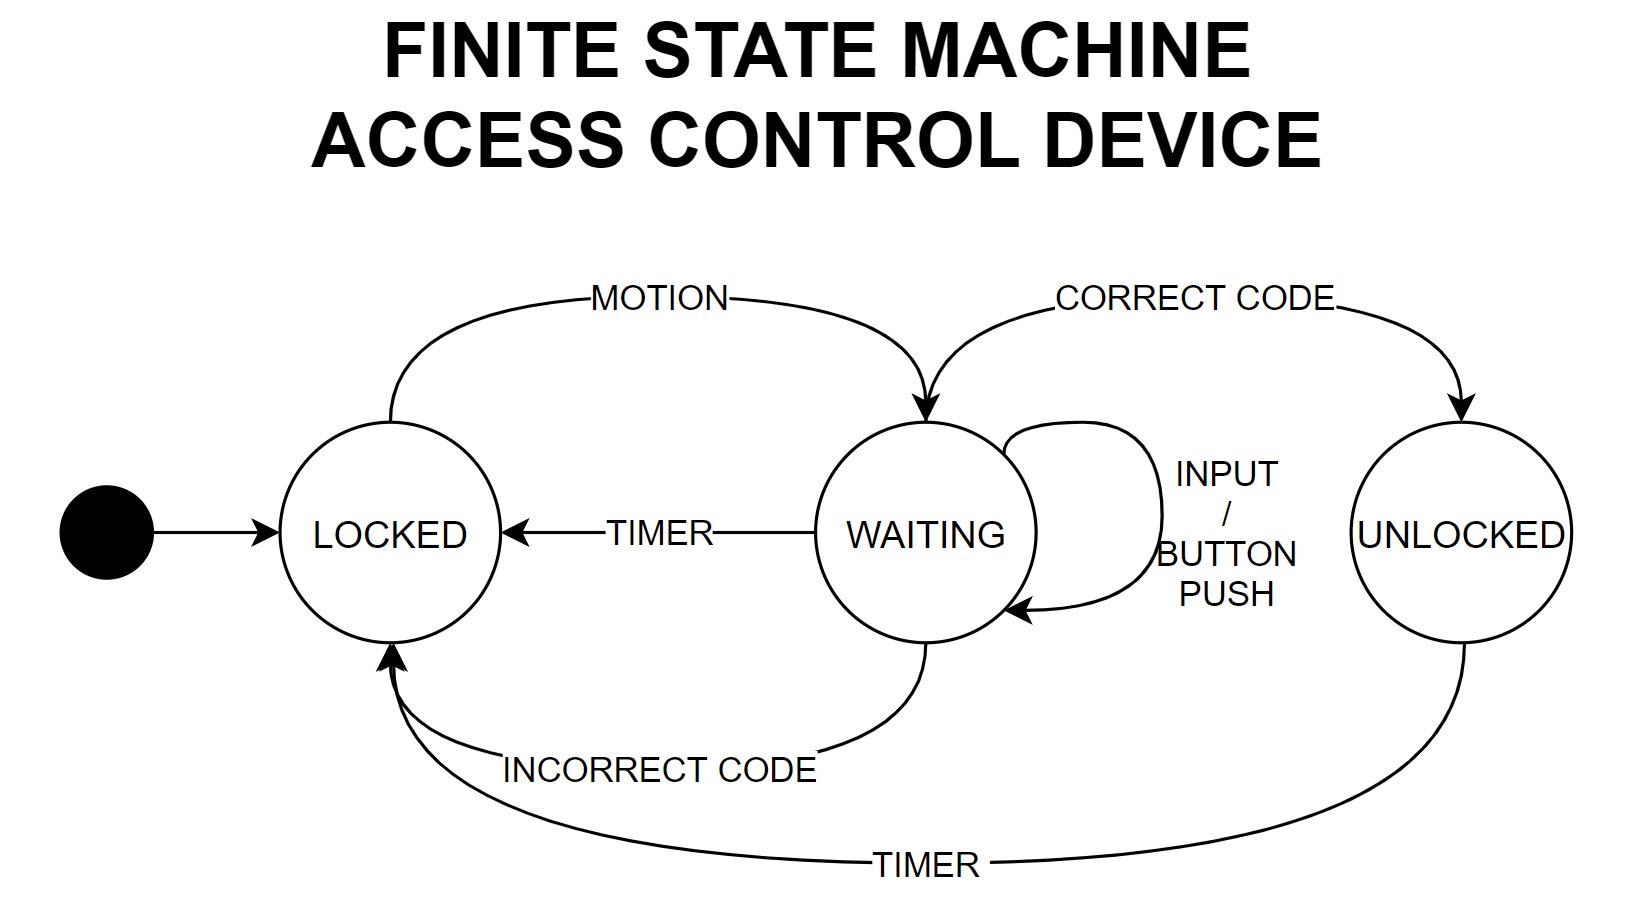
\includegraphics[scale=0.5]{figs/FNS.png}
  \caption{Finite state machine model of access control device}
  \label{fig:framework}
\end{figure}

Design model of ACD was based on the description of functional requirements of the part A. The model contains three states, initial state that is set to locked. Waiting state where input of the access code is taking place. Unlocked state is when entered access code is correct. 
\newline

Motion action is the only thing that can cause the system to go over in waiting state, where access code is entered. That is also the reason behind input loop at waiting state. Further waiting state will go back to locked state if the access code is incorrect, or if the timer ran out and triggered system (optional function). Otherwise, if access code is correct the system is put in unlocked mode, where there’s also a timer that can after an amount of time put the system in locked state.
\newline

Design of the model is drawn as a finite state machine using drawIO UML notation. Where during planning three states, and common main methods of system was taken into account. Input loop at waiting state may seem redundant but describes and helps for the implementation of actual ACD. 


